\section{Ex2.07 Plotting $\sin(x)/x^n$}\label{sec:Plotting_sin}

\subsection{Testo esercizio}
La funzione $g(x;n)$ è data come 
$$g(x;n) = \dfrac{\sin(x)}{x^n}$$

\begin{itemize}
    \item[a)] Creare una funzione $gvalue(x;n)$ che restituisce il valore di $g(x;n)$.
    
    \item[b)] Usa questa funzione per tracciare $$g_1=\dfrac{\sin(x)}{x},\quad 
    g_2=\dfrac{\sin(x)}{x^2}, \quad g_3=\dfrac{\sin(x)}{x^3}$$ nello stesso 
    grafico per $-5<x<5$.
\end{itemize}

\subsection{Svolgimento}
L'esercizio \'e stato semplice. Inizialmente avevo inserito $\rho=7500$ direttamente 
dentro la funzione, successivamente ho reputato opportuno inserire il dato via argomenti 
per rendere la funzione utile per qualsiasi tipo di sfera.

\subsection{Risultato}
\begin{figure}[h]
    \centering
    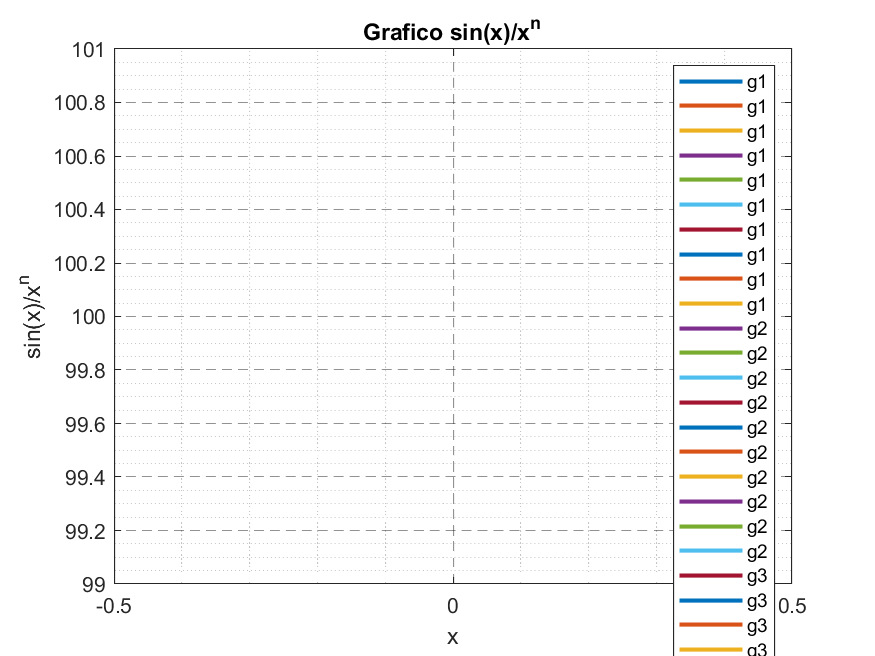
\includegraphics{cap/Elementary/img/script207}
    \GraphCap{$\sin(x)/x^n$}
    \label{fig:script207}
\end{figure}

\subsection{Codice esercizio}
\lstinputlisting[caption = {\nameref{fnc:gvalue}},
linerange={1-3}]
{cap/Elementary/src/function/gvalue.m}

\lstinputlisting[title = {Script Ex2.07}
,linerange={3-22}]
{cap/Elementary/src/script/script207.m}